\documentclass{standalone}
\usepackage{tikz}

\usetikzlibrary{calc,math}


\begin{document}

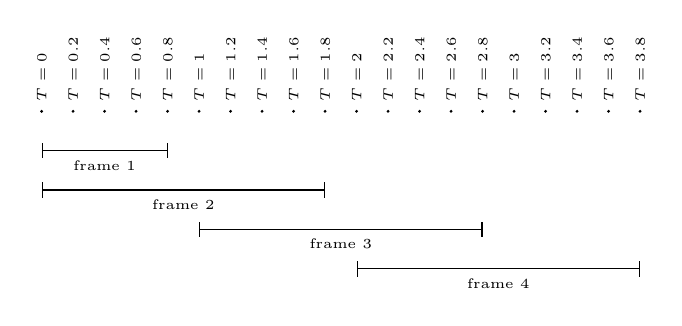
\begin{tikzpicture}
  \pgfkeys{/pgf/number format/.cd,fixed,precision=2}
  \foreach[evaluate={\i / 5} as \x,evaluate={\i / 10} as \t] \i in {0,2,...,39} {
    \draw (\x,0) circle [radius=0.01] node[right,rotate=90,font=\tiny] {$T=\pgfmathprintnumber{\t}$};
  }
  \draw[|-|] (0,-0.5) -- ++(1.6,0) node[below,midway,font=\tiny] {frame 1};
  \draw[|-|] (0,-1) -- ++(3.6,0) node[below,midway,font=\tiny] {frame 2};
  \draw[|-|] (2,-1.5) -- ++(3.6,0) node[below,midway,font=\tiny] {frame 3};
  \draw[|-|] (4,-2) -- ++(3.6,0) node[below,midway,font=\tiny] {frame 4};
\end{tikzpicture}

\end{document}